\section{Webservices}

Many data sources are available on the Internet.  You've probably used
a web browser interface to search through some of this data and even
download it to your computer.  As you may have noticed, this manual
process is labor intensive, error prone, and hard to document.

To provide programmatic and automatic interaction with these data stores, many
websites serve this information through a documented application programmer
interface (API).\footnote{For several examples see the Appendix.}  These
webservice APIs provide a mechanism to create new functionality on top
of existing webcontent.

While there are several ways to implement webservices,
\href{http://en.wikipedia.org/wiki/Representational_state_transfer}{Representational
State Transfer (REST)} has gained widespread popularity.  REST is more of a
style than a standard.  A system designed in the REST style is called RESTful.
RESTful systems typically use HTTP requests to query and post data using the
standard HTTP verbs (GET, POST, PUT, DELETE, etc.).  Often some form of
authentication is necessary to communicate with a webservice.  It is common to
use \href{http://en.wikipedia.org/wiki/OAuth}{OAuth} for this purpose.

\section{Data serialization}

When you use a web browser to view a webpage, your browser handles the HTTP
communication for you.  You specify what you wish to view in the form of a
\href{http://en.wikipedia.org/wiki/Uniform_resource_identifier}{URI} such as
\url{http://example.org/absolute/URI/with/absolute/path/to/resource.txt}.  At
this point your browser communicates with the webserver and requests the
resource.  The resource is typically provided to your web browser as an
\href{http://en.wikipedia.org/wiki/HTML}{HTML} document, which browsers are
specifically designed to render.

Similarly, you will use HTTP to communicate with the Twitter webservice.
However rather than passively consuming webpages, you will be interested in
retrieving data in a form that is amenable to further processing.

Data serialization refers to the process of encoding data structures and
objects in a format that can be used to store this information on disk or
transmit it over the web.  For example, in R you can use the Rdata format to
save R objects to disk and reload them later.  For webservices, JSON and XML
are standard formats.  To better understand this, let's briefly look at data
serialization more generally.

\subsection*{Python object}
First let's create a Python object.
<< d['src/serialize.py|idio|pycon|pyg|l']['mydict'] >>

And let's print the results:
<< d['src/serialize.py|idio|pycon|pyg|l']['pprint'] >>

\subsection*{XML}

How does this object look if we convert it to XML?\footnote{This functionality
is not part of the standard library.  And should not be used in practice.}

<< d['src/serialize.py|idio|pycon|pyg|l']['xml'] >>

\subsection*{JSON}
What if we convert it to JSON?
<< d['src/serialize.py|idio|pycon|pyg|l']['json'] >>

\subsection*{YAML}
What if we convert it to YAML?
<< d['src/serialize.py|idio|pycon|pyg|l']['yaml'] >>

\subsection*{Questions}
Looking over the output of the above formats you should notice several things.

\begin{itemize}
\item Which of the formats uses the largest number of characters?
\item Which uses the fewest?
\item Which looks most like Python?
\end{itemize}

\subsection*{Saving JSON and CSV}
For this project you will be querying the Twitter webservice and will
be getting responses in the JSON format.  After you get your response,
you will want to save it to disk.  I recommend that you use the JSON
format as your main data storage format for this project.

<< d['src/serialize.py|idio|pycon|pyg|l']['savejson'] >>

If you decide that you would like to use R for part of your analysis or for
creating figures, I recommend saving the information you want to work with in R
as a CSV file.  Your JSON file will have nested and non-homogeneous structure,
which is not possible to directly store using CSV.  So you will need to first
decide what data you want to save as CSV and then transform the JSON data into
the necessary form.  Here is an example of how you might transform
\texttt{mydict} above into a list of equal length tuples.

<< d['src/json2csv.py|idio|l']['prepcsv'] >>

Before I can use list comprehension to form the list of tuples I ensure that
the nested structure that I iterate over has equal depth in each substructure.
Then I save the list of tuples as a CSV file.

<< d['src/json2csv.py|idio|l']['savecsv'] >>


\section{Example: US Senate tweets}

If we are interested in Tweets from members of the U.S.
Senate,\footnote{\url{https://twitter.com/gov/lists/us-senate/members}} we
could start by getting a list of their Twitter
accounts.\footnote{\url{https://dev.twitter.com/rest/reference/get/lists/members}}
Then we could retrieve each Senator's user
profile,\footnote{\url{https://dev.twitter.com/rest/reference/get/statuses/user_timeline}}
which contains their most recent tweets.  This information could then be used
to create a document-term matrix where a document is defined as a senator's
recent tweets.  To try to visualize this data we might project the
document-term matrix onto its first and second principal components.  At this
point, it would be useful to have additional data about each senator (e.g.,
party affiliation, years in
office).\footnote{\url{https://sunlightlabs.github.io/congress/}}

In the appendix, you will find a script to do the above data gathering and
exploration. This should give you a sense of how you might go about collecting
your data.  For additional examples see \cite{russell2013mining}.

\newpage
\section*{Appendix}

\subsection*{Code}

<< d['src/senators.py|pyg|l'] >>

\begin{figure}[h]
\centering
  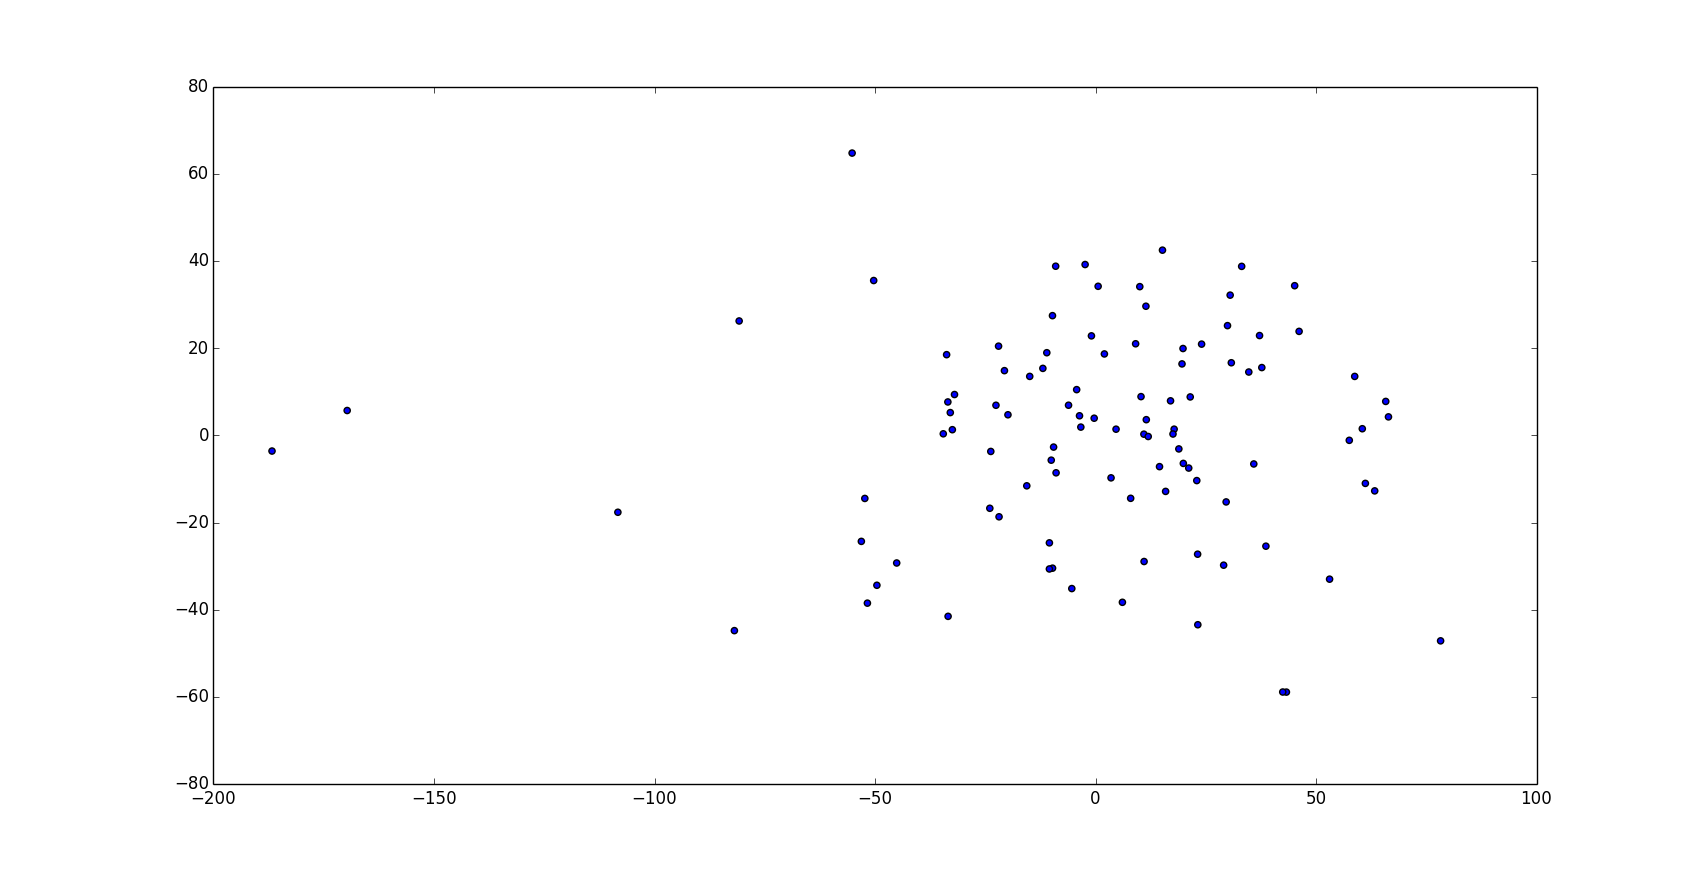
\includegraphics[width=0.9\linewidth]{fig/pca.png}
  \caption{Document-term matrix projected on first and second principal axes.}\label{fig:pca}
\end{figure}

\subsection*{Links}

\subsubsection*{Webservices} 
% add science resources
\begin{itemize}
\item \url{https://dev.twitter.com/overview/documentation}
\item \url{https://developers.facebook.com/docs/graph-api}
\item \url{https://developers.google.com/youtube/getting_started}
\item \url{http://en.wikipedia.org/w/api.php}
\item \url{http://www.mediawiki.org/wiki/API:Main_page}
\item \url{https://developer.github.com/v3/}
\end{itemize}

\subsubsection*{Serialization}

\begin{itemize}
\item \url{http://en.wikipedia.org/wiki/Serialization}
\item \url{http://en.wikipedia.org/wiki/Comparison_of_data_serialization_formats}
\item \url{http://www.json.org/xml.html}
\item \url{http://yaml.org/}
\item \url{http://www.drdobbs.com/web-development/after-xml-json-then-what/240151851}
\item \url{http://www.cowtowncoder.com/blog/archives/2012/04/entry_473.html}
\end{itemize}

\bibliographystyle{plain}
\bibliography{lecture}
